\documentclass[tikz,10pt]{standalone}
\usepackage{newtxtext,newtxmath}

\usetikzlibrary{decorations}
\usetikzlibrary{calc,positioning}
\usetikzlibrary{decorations.pathmorphing}

% Define sizes in cm
\def\totalwidth{15.92}
\def\totalheight{4}
\def\widthA{5.31}
\def\widthB{5.30}
\def\widthC{5.31}



\makeatletter
\pgfdeclareshape{cavity}
{
    \inheritsavedanchors[from=rectangle]
    \inheritanchorborder[from=rectangle]
    \inheritanchor[from=rectangle]{north}
    \inheritanchor[from=rectangle]{north west}
    \inheritanchor[from=rectangle]{north east}
    \inheritanchor[from=rectangle]{center}
    \inheritanchor[from=rectangle]{west}
    \inheritanchor[from=rectangle]{east}
    \inheritanchor[from=rectangle]{mid}
    \inheritanchor[from=rectangle]{mid west}
    \inheritanchor[from=rectangle]{mid east}
    \inheritanchor[from=rectangle]{base}
    \inheritanchor[from=rectangle]{base west}
    \inheritanchor[from=rectangle]{base east}
    \inheritanchor[from=rectangle]{south}
    \inheritanchor[from=rectangle]{south west}
    \inheritanchor[from=rectangle]{south east}
    \inheritbackgroundpath[from=rectangle]
    \foregroundpath{
      %  \centerpoint
        \pgf@xc=\pgf@x
        \pgf@yc=\pgf@y
        \pgfpathmoveto{\pgfpoint{\pgf@xc-0.5}{\pgf@yc+0.5}}
        \pgfpathlineto{\pgfpoint{\pgf@xc-0.5}{\pgf@yc-0.5}}
        \pgfpathlineto{\pgfpoint{\pgf@xc+0.8}{\pgf@yc-0.5}}
        \pgfpathlineto{\pgfpoint{\pgf@xc+0.5}{\pgf@yc+0.5}}
        \pgfpathlineto{\pgfpoint{\pgf@xc-0.5}{\pgf@yc+0.5}}
        \pgfclosepath
        \pgfsetfillcolor{\pgfkeysvalueof{/tikz/mirror fill}}
        \pgfusepath{fill}
    }
}
\makeatother

\pgfkeyssetvalue{/tikz/mirror fill}{black!50}
\pgfkeyssetvalue{/tikz/cavity inner color}{white}
\pgfkeyssetvalue{/tikz/cavity outer color}{red!40}


\tikzstyle{dot}                  = [draw,fill=black,anchor=center,
                                    minimum width=1.5cm,minimum height=2pt,
                                    inner sep=0pt,outer sep=0pt]
\tikzstyle{electron}[red]        = [shading=ball,ball color=#1, 
                                    circle,minimum size=5mm]

\tikzset{photon/.style={decoration={snake,pre length=3pt,post length=5pt},
                        decorate, very thick, -latex}
}
\tikzstyle{ket}                  = [left,inner sep=3pt]
\tikzstyle{letter}               = [anchor=north west,inner sep=0pt]

\begin{document}
    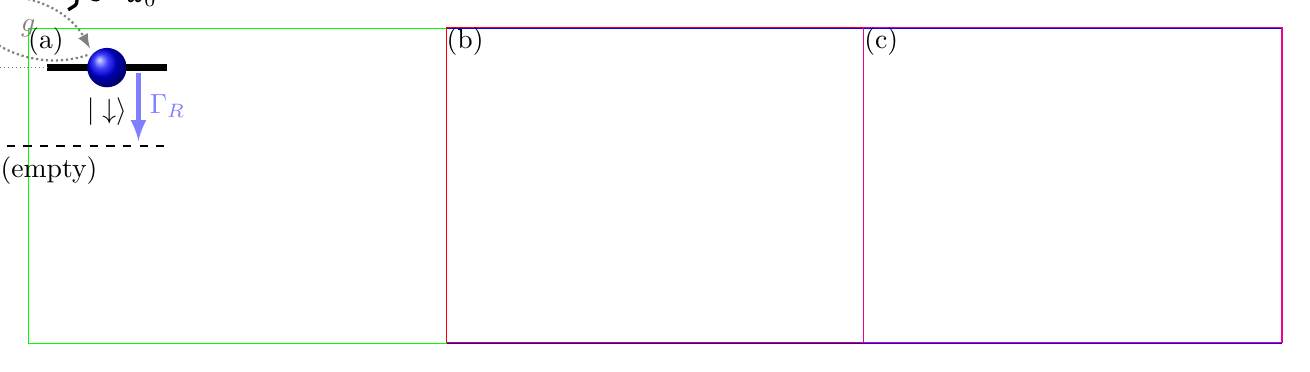
\begin{tikzpicture}[]
        \useasboundingbox[draw,blue] (0,0) rectangle (\totalwidth,-\totalheight);
        
        % Part (a)
        \begin{scope}[local bounding box=A]
            \useasboundingbox[draw,green] (0,0) rectangle (\widthA, -\totalheight);

	        % Letter
            \node[letter] at (current bounding box.north west) {(a)} ;

            \begin{scope}[shift={(A.center)}]
                
            \end{scope}
        \end{scope}

        % Part (b)
        \begin{scope}[shift={($(current bounding box.north west)!\widthA/\totalwidth!(current bounding box.north east)$)}, local bounding box=B]
            
            \useasboundingbox[draw,red] (0,0) rectangle (\widthB, -\totalheight);

            % Letter
            \node[letter] at (0,0) {(b)} ;

            \begin{scope}[shift={(B.center)}]
            \end{scope}
        \end{scope}

        % Part (c)
        \begin{scope}[shift={($(current bounding box.north east)!\widthC/\totalwidth!(current bounding box.north west)$)}, local bounding box=C]
            \useasboundingbox[draw,magenta] (0,0) rectangle (\widthC, -\totalheight);

            % Letter
            \node[letter] at (0,0) {(c)} ;

            \begin{scope}[shift={(C.center)}]
                \coordinate (up)   at (-1,0.5);
                \coordinate (down) at (1,-0.5);

                \node[dot] (U) at (up)   {};
                \node[dot] (D) at (down) {};
                \node[electron=red, label={above:$|\uparrow\rangle$}  ] (up) at  (up) {};
                \node[electron=blue,label={below:$|\downarrow\rangle$}] (down) at (down) {};

                \draw[thick,dashed] (-1.75,-1.5) --++ (3.5,0) 
                      node[pos=0.1,inner sep=0pt] (Gu)  {}
                      node[midway,below] {$|0\rangle$ (empty)}
                      node[pos=0.9,inner sep=0pt]   (Gd)  {};
                \draw[-latex,shorten <=2pt,shorten >=2pt,thick,densely dotted,gray] (up.south east) to[bend left=40] (down.north west)
                    edge[bend left=40] (up.south east);
                \node[at={($(up)!0.5!(down)$)},gray,minimum width=1cm] (g) {$g$};
                \draw[photon] (g.north east) -- (30:2) 
                      node[midway, below right] {$\omega_0$}
                      node[at end] (ph) {};

                \draw[thin,gray,densely dotted] (U.west) --++ (-0.75,0);
                \draw[thin,gray,densely dotted] (D.west) --++ (-2.75,0) node[pos=0.8,inner sep=0] (C) {};
                \draw[->,>=latex,shorten <=1pt,shorten >=1pt,ultra thick,red!50] (Gu.north) -- (Gu.north|-up)
                      node[near start,right] {$\Gamma_L$};
                \draw[<-,>=latex,shorten <=1pt,shorten >=2pt,ultra thick,blue!50] (Gd.north) -- (Gd.north|-down)
                      node[midway,right] {$\Gamma_R$};
                \draw[<->,>=latex,thin,densely dotted,gray] (C.north) -- (C.north|-up) node[midway,left] {$\Delta\epsilon$};
            \end{scope}
        \end{scope}
    \end{tikzpicture}
\end{document}

